\documentclass{beamer}
\mode<presentation>
\usepackage{amsmath}
\usepackage{amssymb}
%\usepackage{advdate}
\usepackage{graphicx}
\graphicspath{{../figs/}}
\usepackage{adjustbox}
\usepackage{subcaption}
\usepackage{enumitem}
\usepackage{multicol}
\usepackage{mathtools}
\usepackage{listings}
\usepackage{url}
\def\UrlBreaks{\do\/\do-}
\usetheme{Boadilla}
\usecolortheme{lily}
\setbeamertemplate{footline}
{
  \leavevmode%
  \hbox{%
  \begin{beamercolorbox}[wd=\paperwidth,ht=2.25ex,dp=1ex,right]{author in head/foot}%
    \insertframenumber{} / \inserttotalframenumber\hspace*{2ex} 
  \end{beamercolorbox}}%
  \vskip0pt%
}
\setbeamertemplate{navigation symbols}{}
\let\solution\relax
\usepackage{gvv}
\lstset{
%language=C,
frame=single, 
breaklines=true,
columns=fullflexible
}

\numberwithin{equation}{section}


\title{4.2.23}
\author{EE25BTECH11020 - Darsh Pankaj Gajare}
\begin{document}
\maketitle
% \newpage
% \bigskip

Question:\\
Show that two lines $a_1x+b_1y+c_1=0$ and $a_2x+b_2y+c_2=0$ where $b_1b_2\neq0$ are perpendicular if $a_1a_2-b_1b_2=0$.\\
\solution
\begin{table}[H]
	\centering
	\caption{}
	\begin{tabular}{|c|c|}
\hline
\textbf{Name} & \textbf{Value} \\
\hline
Circle & $\vec{x}^\top\vec{x} - a^2 = 0$ \\
\hline
Line & $\vec{x} = \myvec{\tfrac{a}{\sqrt{2}} \\ 0} + \kappa\myvec{0 \\ 1}$ \\
\hline
\end{tabular}

	\label{}
\end{table}

For the lines to be perpendicular, their normals must be orthogonal:
\begin{align}
    \vec{n_1}^\top \vec{n_2} &= 0
\end{align}

Evaluating the product,
\begin{align}
    \myvec{a_1 & b_1}\myvec{a_2 \\ b_2}=0 
\end{align}
\textbf{Example:}
Let us assume the values $a_1=2$, $a_2=3$, $b_1=3$, $b_2=2$, $c_1=2$ and $c_2=3$
Plot using C libraries:
\begin{figure}[H]
	\centering
	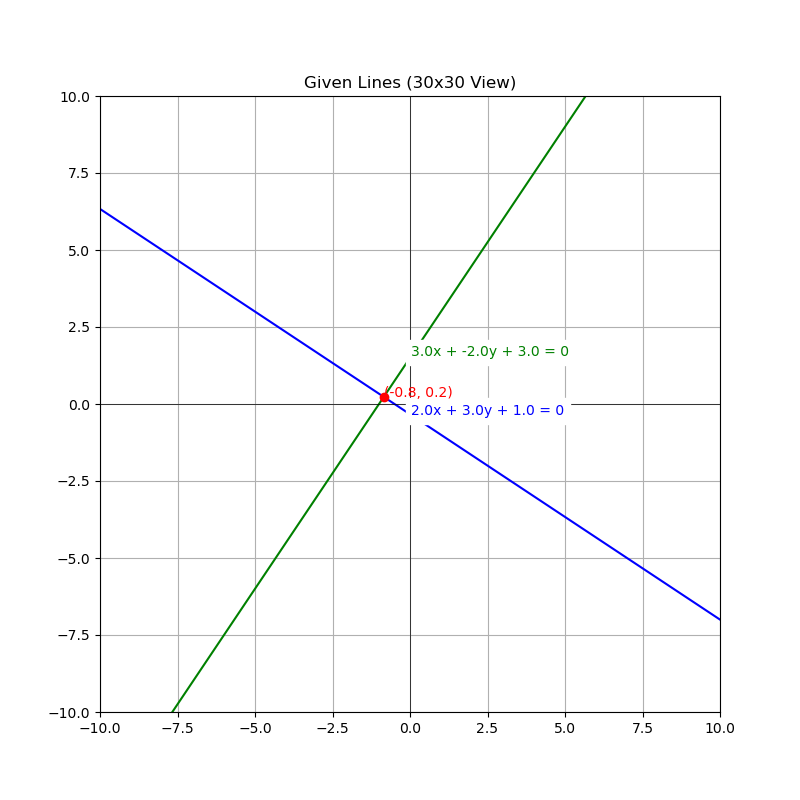
\includegraphics[scale=0.5]{img}
	\caption*{}
	\label{img1}
\end{figure}
Plot using Python:
\begin{figure}[H]
	\centering
	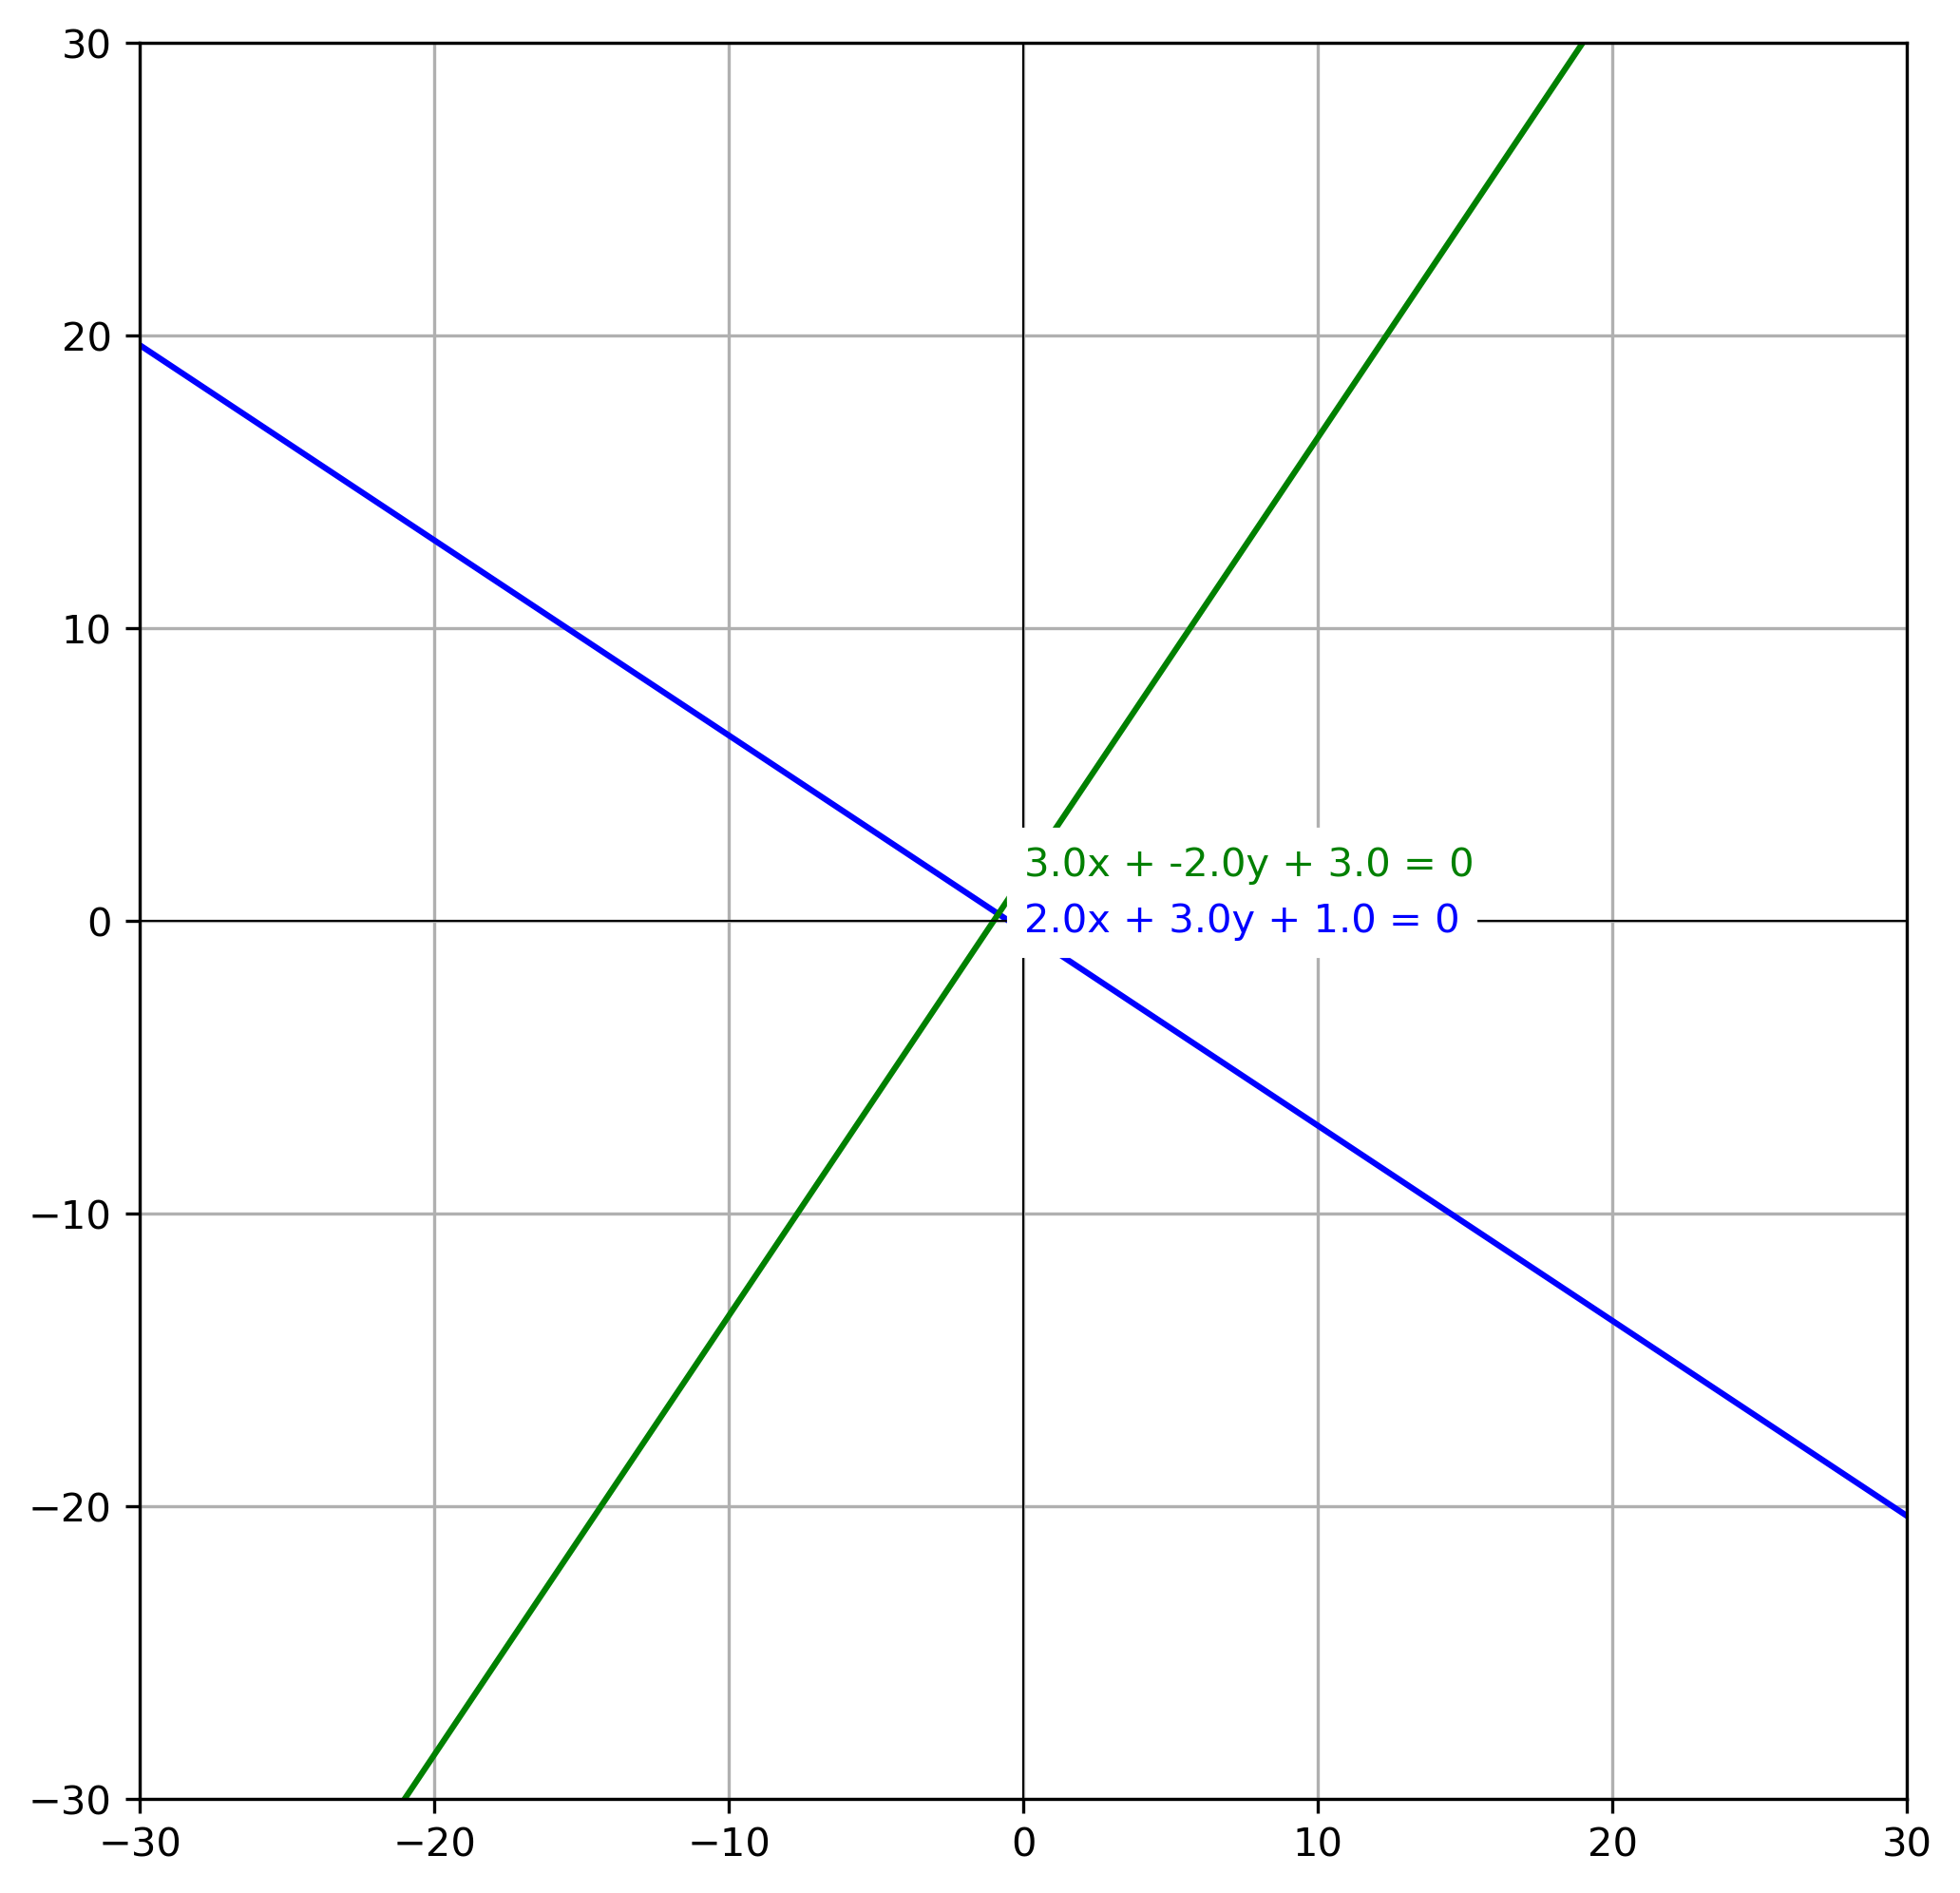
\includegraphics[scale=0.5]{img1}
	\caption*{}
	\label{img2}
\end{figure}
\end{document}

